\section{}

\textbf{Tiempo de lectura:} \{s08-reading-time\}

Ya hemos discutido anteriormente acerca de los componentes más comunes
en un sistema operativo (véase el
\hyperref[componentes_del_sistema]{???}). En esta sección comentaremos
cómo se clasifican los distintos sistemas operativos según la
organización e interconexión de sus componentes.

\section{Estructura sencilla}\label{_estructura_sencilla}

{} Los sistemas con \textbf{estructura sencilla} se caracterizan por:

\begin{itemize}
\item
  No tener una estructura bien definida. Los componentes no están bien
  separados y las interfaces entre ellos no están bien definidas.
\item
  Son sistemas \textbf{monolíticos}, dado que gran parte de la
  funcionalidad del sistema se implementa en el núcleo.
\end{itemize}

En la actualidad, este tipo de estructura se usa en sistemas que deben
ejecutarse en hardware muy limitado, como en sensores conectados,
termostatos, sistemas de control o electrodomésticos.

\subsection{MS-DOS}\label{_ms_dos}

Por ejemplo, en el \{msdos\} los programas de aplicación podían acceder
directamente a toda la memoria y a cualquier dispositivo. Disponiendo de
esa libertad un programa erróneo cualquiera podía corromper el sistema
completo.

\begin{figure}
\centering
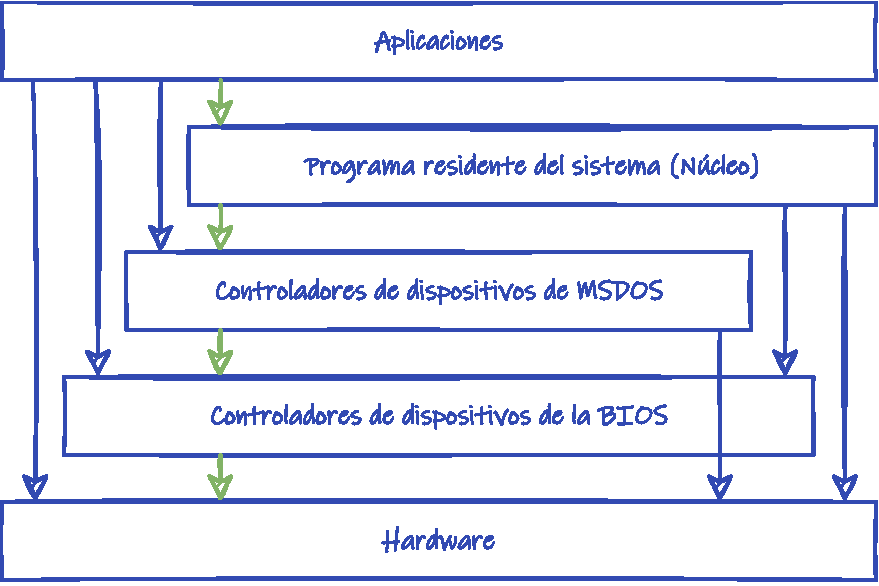
\includegraphics[width=0.8\textwidth]{media/C08_estructura/estructura_msdos.pdf}
\caption{Esquema de la estructura de
MS-DOS.}\label{fig-estructura-msdos}
\end{figure}

Como el \{intel8086\} para el que fue escrito MS-DOS no proporcionaba un
modo dual de operación, los diseñadores del sistema no podían evitar que
los programas de usuario accedieran directamente al hardware ni tenían
forma de proteger las distintas partes del sistema operativo.

\subsection{UNIX}\label{_unix}

Otro ejemplo es el de \href{https://es.wikipedia.org/wiki/Unix}{UNIX
original}, donde sí había una separación clara entre procesos de usuario
y código del sistema, pero juntaba mucha funcionalidad en el núcleo del
sistema.

\begin{figure}
\centering
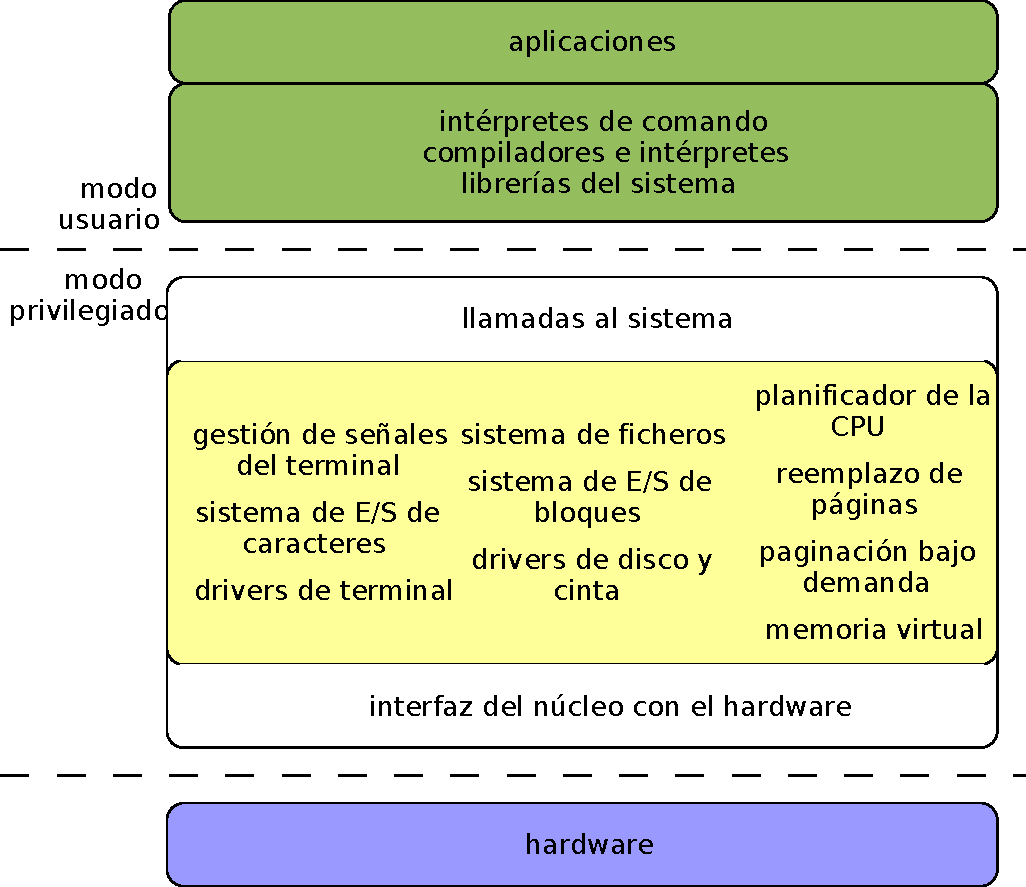
\includegraphics[width=0.8\textwidth]{media/C08_estructura/estructura_unix.pdf}
\caption{Esquema de la estructura de UNIX.}\label{fig-estructura-unix}
\end{figure}

El núcleo proporciona la planificación de CPU, la gestión de la memoria,
el soporte de los sistemas de archivos y muchas otras funcionalidades
del sistema operativo. En general se trata de una enorme cantidad de
funcionalidad que es difícil de implementar y mantener, si no se
compartimenta adecuadamente.

Tanto MS-DOS como UNIX eran originalmente sistemas pequeños y simples,
limitados por las funcionalidades del hardware de su época, que fueron
creciendo más allá de las previsiones originales. Lo cierto es que con
mejor soporte del hardware se puede dividir el sistema operativo en
piezas más pequeñas y apropiadas que las del MS-DOS y el UNIX original.

\section{Estructura en capas}\label{_estructura_en_capas}

{} Los sistemas con \textbf{estructura en capas} se caracterizan por:

\begin{itemize}
\item
  La funcionalidad se divide en capas, de tal forma que una capa solo
  utiliza funciones y servicios de la capa inmediatamente inferior y lo
  hace a través de una interfaz bien definida.
\item
  Como en la programación orientada a objetos, cada capa oculta a la
  capa superior los detalles de su implementación. Por ejemplo, las
  estructuras de datos internas que usa y las operaciones o el hardware
  de la capa inferior que utiliza.
\item
  Escalan mejor que los sistemas con \textbf{estructura sencilla} porque
  las capas hacen que el código esté mejor compartimentado. Por ejemplo,
  al corregir un \emph{bug} o añadir una nueva funcionalidad solo hay
  que preocuparse de su efecto en la capa a la que afecta y no en todo
  el código del núcleo ---siempre que no se altere la interfaz de la
  capa con el exterior---.
\item
  Ser menos eficiente que la de los sistemas de \textbf{estructura
  sencilla}. En cada capa los argumentos son transformados y los datos
  necesarios deben de ser transferidos al invocar operaciones en la capa
  inferior, por lo que cada una añade cierto nivel de sobrecarga al
  funcionamiento del sistema.
\item
  También son sistemas \textbf{monolíticos}, dado que gran parte de la
  funcionalidad del sistema se implementa en el núcleo, aunque ahora el
  núcleo esté compartimentado en capas.
\end{itemize}

Actualmente, no existe ningún motivo para diseñar sistemas operativos
con esta estructura. Es preferible utilizar la \textbf{estructura
modular}, que presenta las mismas ventajas y evita las dificultades en
el diseño, de las que hablaremos a continuación.

Un ejemplo de este tipo de sistemas operativos es el \{os2\}.

\begin{figure}
\centering
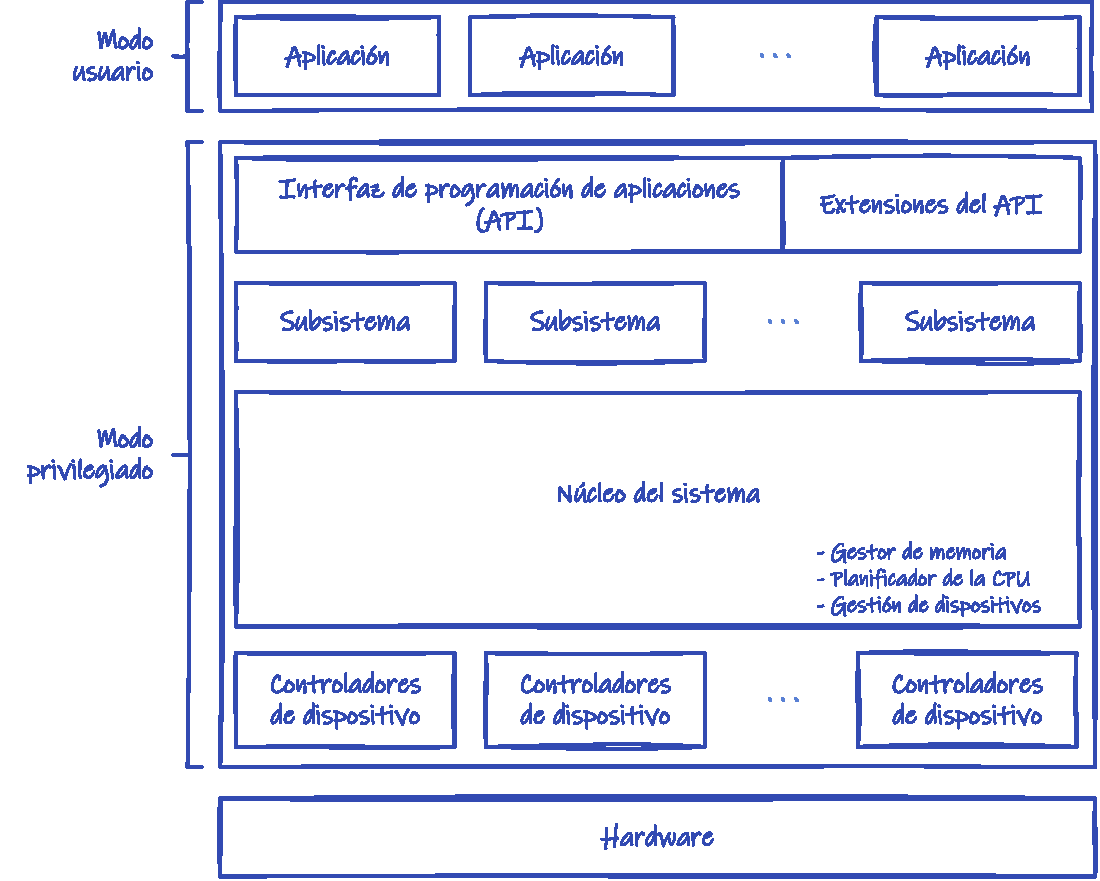
\includegraphics[width=0.8\textwidth]{media/C08_estructura/estructura_os2.pdf}
\caption{Esquema de la estructura de IBM
OS/2.}\label{fig-estructura-os2}
\end{figure}

\subsection{Dificultades con el
diseño}\label{_dificultades_con_el_diseuxf1o}

Es importante tener en cuenta que diseñar un sistema con
\textbf{estructura en capas} no es tan sencillo como pudiera parecer. La
definición de las capas y sus funcionalidades debe ser planificada
cuidadosamente debido a la restricción, comentada anteriormente, de que
una capa solo puede utilizar los servicios de las capas inferiores.

Por ejemplo, el planificador de la CPU suele tener información de los
procesos que están en la memoria. Parte de esa información puede ser
almacenada en el disco para aumentar la memoria principal disponible.
Esto nos debería llevar a pensar que la gestión del almacenamiento
secundario debe ir en una capa inferior a la del planificador de la CPU,
para que así el segundo pueda pedir al primero que guarde los datos en
disco.

Sin embargo, el planificador de la CPU debe asignar la CPU a otro
proceso cuando el proceso que actualmente la ocupa solicita alguna
operación de E/S ---lo típico en multiprogramación---. Como es la
gestión del almacenamiento secundario el que debe pedir una operación al
planificador de la CPU, ahora el primero debe estar sobre el segundo.

La solución a esta dependencia circular es hacer que ambos componentes
estén en la misma capa. Este tipo de dependencias no son raras, ocurre
en muchos otros casos, ya que los componentes del sistema operativo
suelen depender mucho unos de otros.

Al final, la solución de compromiso es tender hacia sistemas con muy
pocas capas donde cada una tiene mucha funcionalidad. Esto limita mucho
las ventajas de esta técnica porque no permite compartimentar el núcleo
tanto como sería deseable.

\section{Microkernel}\label{_microkernel}

{} {} Los sistemas con \textbf{estructura microkernel} se caracterizan
por:

\begin{itemize}
\item
  Eliminar todos los componentes no esenciales del núcleo e
  implementarlos como procesos de usuario.
\item
  Un núcleo \textbf{microkernel} proporciona funciones mínimas de
  gestión de procesos y de memoria y algún mecanismo de comunicación
  entre procesos. Sin embargo, hay que tener en cuenta que hay poco
  consenso a este respecto, por lo que algunos \textbf{microkernel}
  reales incluyen en el núcleo algunas funcionalidades adicionales.
\item
  El mecanismo de comunicación permite a los procesos de los usuarios
  solicitar servicios a los componentes del sistema. También sirve para
  que los componentes del sistema se comuniquen entre sí y se pidan
  servicio.
\end{itemize}

Aunque se puede utilizar en cualquier ámbito, este tipo de estructura se
utiliza, principalmente, en algunos sistemas operativos para sistemas
empotrados, como ocurre con los de \textbf{estructura simple}. Sin
embargo, la \textbf{estructura microkernel} necesita un hardware algo
más potente, que admita modo dual de operación; siendo especialmente
interesante en sistemas críticos o cuando hay especial preocupación por
la seguridad. Algunos ejemplos son los sistemas de automoción o los
equipos médicos.

Dado que los componentes del sistema están aislados unos de otros ---ya
que se implementan como procesos de usuario--- el mecanismo de
comunicación entre procesos es la única forma que tienen los procesos de
los usuarios y los componentes, de solicitarles un servicio.

\begin{figure}
\centering
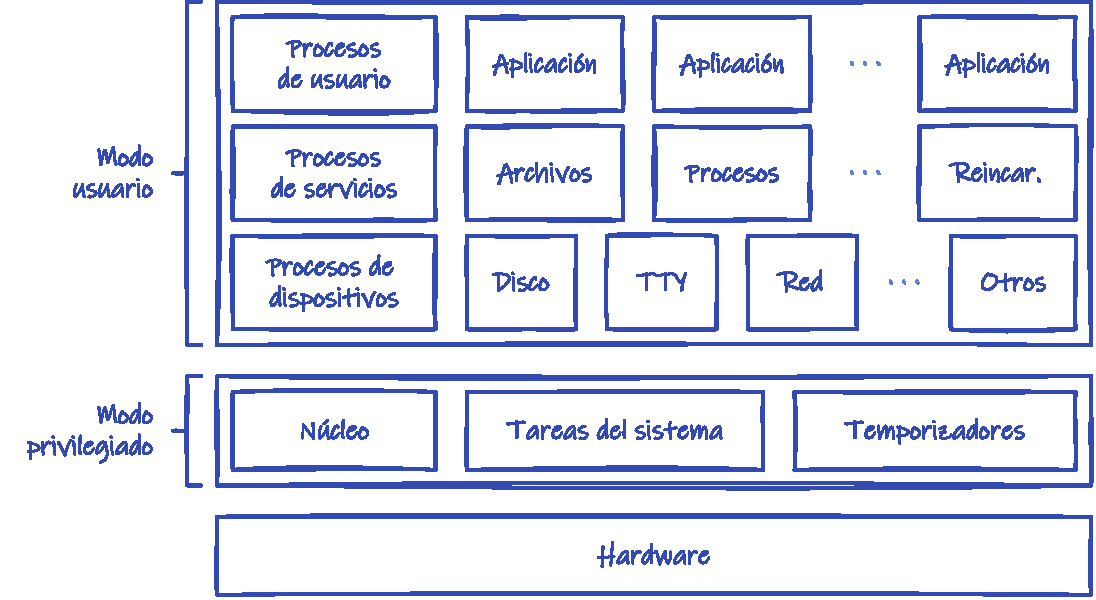
\includegraphics[width=0.8\textwidth]{media/C08_estructura/estructura_minix3.pdf}
\caption{Esquema de la estructura microkernel de MINIX
3.}\label{fig-estructura-minix3}
\end{figure}

Generalmente esta comunicación se implementa mediante paso de mensajes
(véase el \hyperref[_comunicaciuxf3n_entre_procesos]{???}).

Entre los beneficios de estos sistemas operativos se incluyen:

\begin{itemize}
\item
  \textbf{Facilidad a la hora de añadir nuevas funcionalidades}. Los
  nuevos servicios son añadidos como aplicaciones de nivel de usuario,
  por lo que no es necesario hacer modificaciones en el núcleo.
  Desarrollar en el modo privilegiado siempre es más peligrosos que en
  el modo usuario porque los errores pueden ser catastróficos: bloqueo o
  caída del sistema, corrupción de datos, etc.
\item
  \textbf{Facilidad a la hora de llevar el sistema a otras plataformas}.
  Puesto que el núcleo es muy pequeño, resulta muy sencillo de portar a
  otras plataformas.
\item
  \textbf{Más seguridad y fiabilidad}. Puesto que la mayor parte de los
  servicios se ejecutan como procesos separados de usuario, un servicio
  que falla no puede afectar a otros ni puede ser utilizado para ganar
  acceso a otros servicios o al núcleo. Además se pueden implementar
  estrategias para mejorar la tolerancia a fallos, como reiniciar un
  servicio que ha fallado, como si fuera un programa cualquiera.
\end{itemize}

\subsection{Rendimiento}\label{_rendimiento}

El mayor inconveniente es el pobre rendimiento que puede tener, causado
por la sobrecarga que añade el mecanismo de comunicación.

Por ejemplo, \{windowsnt\} nació con una estructura de
\textbf{microkernel} en capas donde una parte importante de los
servicios eran proporcionados por unos procesos de usuario llamados
subsistemas.

El sistema operativo podía mostrar diferentes personalidades o
\emph{entornos operativos} ---básicamente de OS/2, POSIX y MS-DOS--- a
través del uso de subsistemas ambientales, que también se ejecutaban
como procesos de usuario. Las aplicaciones de Microsoft Windows NT se
comunicaban con estos subsistemas utilizando un mecanismo de
comunicación denominado
\href{https://en.wikipedia.org/wiki/Local_Inter-Process_Communication}{LPC}
(\emph{Local Inter-Process Communication}).

Con esta estructura, la pérdida de rendimiento respecto a Microsoft
Windows 95 era tan importante ---especialmente en lo relativo a
operaciones gráficas--- que los diseñadores se vieron obligados a mover
más servicios al espacio del núcleo en la versión 4.0. El resultado es
que los Windows sucesores a Windows NT 4.0 tienen una arquitectura más
monolítica que microkernel, ya que aunque muchos servicios siguen siendo
proporcionados por procesos de usuario, esto solo ocurre con aquellos
donde el rendimiento no es un factor crítico.

Microsoft Windows XP tiene 280 llamadas al sistema a las que hay que
sumar las más de 650 llamadas del subsistema gráfico, que también se
aloja en el núcleo desde Microsoft Windows NT 4.0. Mientras que
Microsoft Windows NT 3.51 tenía algo menos de 200 llamadas al sistema.

Sin embargo, varios sistemas operativos siguen utilizando núcleos
\textbf{microkernel}, como \{qnx\} o \{minix3\}. Ambos son sistemas
operativos de tiempo real, que basan en la estructura de
\textbf{microkernel} su estabilidad como sistema para tareas críticas.

En la \hyperref[fig-estructura-minix3]{Esquema de la estructura
microkernel de MINIX 3.}, por ejemplo, se puede observar un esquema de
\{minix3\}. El núcleo es muy pequeño ---apenas tiene 5000 líneas de
código--- por lo que la mayor parte de la funcionalidad reside en los
procesos de servicios y de controladores de dispositivo.

\{minix3\} es un sistema compatible POSIX. Así que soporta las llamadas
al sistema definidas por este estándar, pero estas se convierten en
mensajes enviados al servidor correspondiente con la petición, y no en
llamadas directas al núcleo. Para que un servidor pueda atender una
petición, quizás tenga que enviar peticiones a otros servidores o
controladores de dispositivo. Incluso pueden tener que hacer llamadas al
núcleo, para solicitar alguna operación privilegiada que no se puede
implementar en el modo usuario. Por ejemplo, operaciones de E/S
---fundamentales para los controladores de dispositivo--- o el acceso a
tablas del núcleo ---como la tabla de procesos---.

Es este trasiego de mensajes con peticiones y respuestas ---y la
correspondiente conmutación de procesos en la CPU para ejecutar el
proceso que atiende cada mensaje--- para resolver una petición de un
proceso de usuario, lo que teóricamente justifica el menor rendimiento
de los sistemas \textbf{microkernel}.

\section{Estructura modular}\label{_estructura_modular}

Los sistemas con \textbf{estructura modular} se caracterizan por:

\begin{itemize}
\item
  Dividir el núcleo en módulos, cada uno de los cuales implementa
  funciones y servicios concretos y se comunican entre sí a través de
  una interfaz bien definida.
\item
  Como en la programación orientada a objetos, cada módulo oculta al
  resto los detalles de su implementación.
\item
  Todos los módulos pueden llamar a funciones de la interfaz de
  cualquier otro módulo, a diferencia de los sistemas operativos con
  \textbf{estructura en capas}, donde una capa solo podía usar a la
  inmediatamente inferior.
\item
  También son sistemas \textbf{monolíticos}, dado que gran parte de la
  funcionalidad del sistema se implementa en el núcleo, aunque ahora el
  núcleo esté compartimentado en módulos.
\end{itemize}

La mayor parte de los sistemas operativos de propósito general, que se
instalan tanto en sistema de escritorio como en servidores, son de este
tipo. También en los \emph{smartphones}, \emph{smart TV} y otros
dispositivos «inteligentes» y, en general, en muchos sistemas
empotrados.

Estos núcleos suelen disponer de un pequeño conjunto de componentes
fundamentales que se cargan durante el arranque. Posteriormente pueden
cargar módulos adicionales, tanto durante la inicialización del sistema
como en tiempo de ejecución.

\begin{figure}
\centering
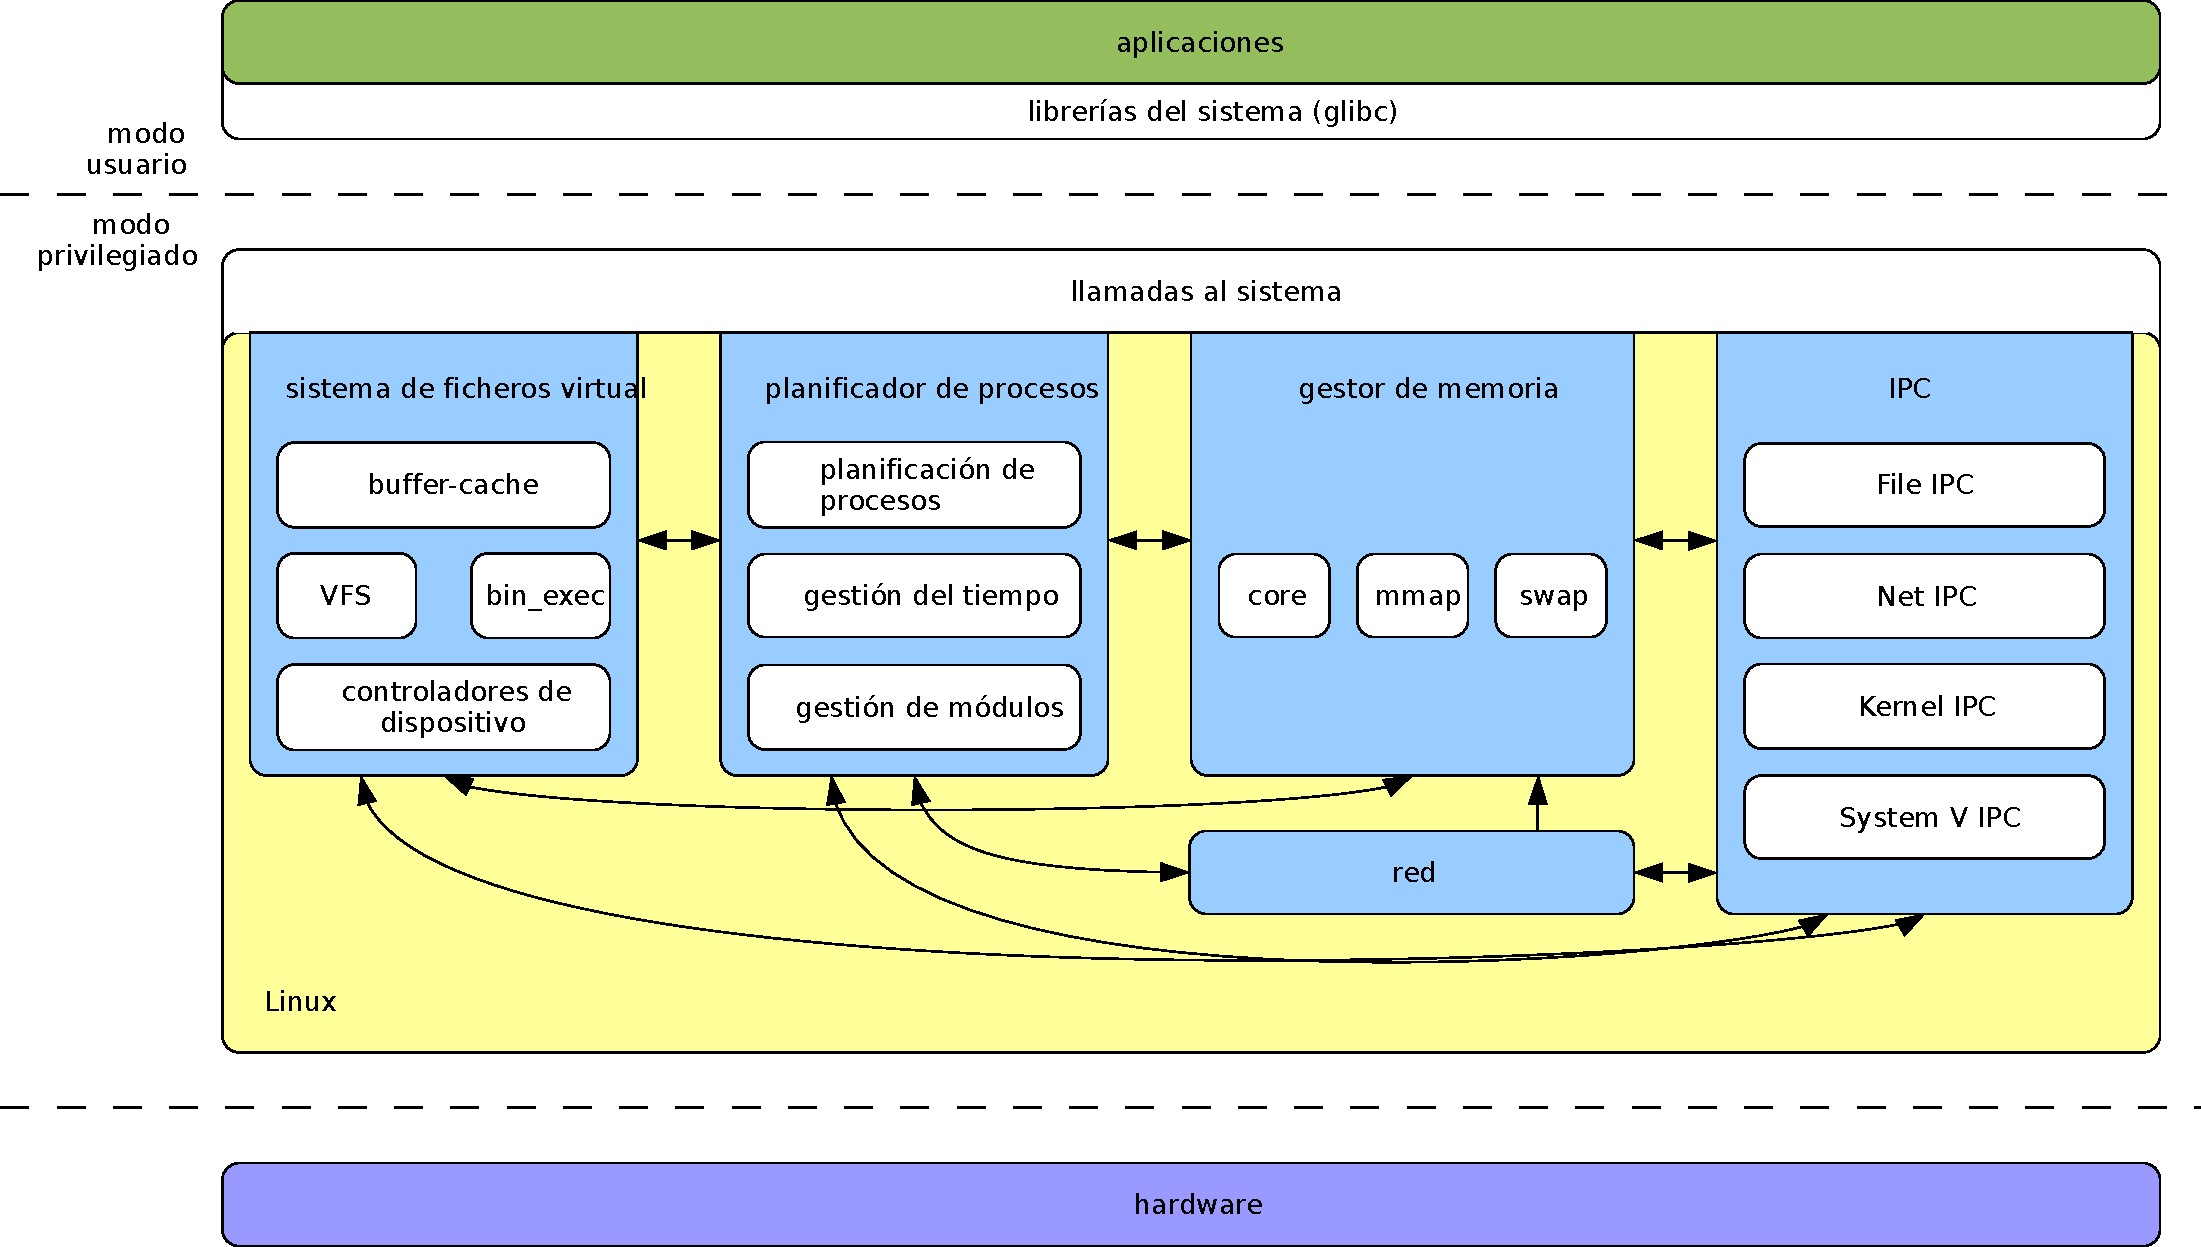
\includegraphics[width=0.8\textwidth]{media/C08_estructura/estructura_linux.pdf}
\caption{Esquema de la estructura del núcleo
Linux.}\label{fig-estructura-linux}
\end{figure}

En este aspecto se asemejan a los núcleos \textbf{microkernel}, ya que
el módulo principal solo tiene funciones básicas. Sin embargo los
núcleos modulares:

\begin{itemize}
\item
  \textbf{Son más eficientes} al no necesitar un mecanismo de
  comunicación, puesto que los componentes se cargan en la memoria
  destinada al núcleo, por lo que pueden llamarse directamente.
\item
  \textbf{Son menos seguros y fiables}, puesto que gran parte de su
  funcionalidad se ofrece desde el modo privilegiado. Un error en
  cualquier componente puede comprometer o hacer caer el sistema.
\end{itemize}

Este tipo de estructura es la utilizada en los UNIX modernos, como
\{solaris\}, \{freebsd\}, \{gnulinux\} (véase la
\hyperref[fig-estructura-linux]{Esquema de la estructura del núcleo
Linux.}) y \{macos\}. También se puede considerar que los sistemas
Windows actuales, tienen estructura modular.
